\chapter{サロゲート最適化}
\label{chap::surrogate}
\hspace{1zw}本章では,最適化を加速させるためのサロゲート最適化の試みについて述べる.
\section{概要}
本章の最適化システムの構成を\figref{fig::surrogate_system}に示す.\chapref{chap::sim}では,設計変数 $\vec{x}$から計算される空調設定温度スケジュール $t_{set}(\vec{x},t)$について,室内快適性$TCFM(\vec{x}, \mathcal{A}, t)$とエネルギー消費量$ASEE(\vec{x},\mathcal{A}, t)$の2つの時系列データをEnergyPlusシミュレーションによって出力し,それら2つの時系列データから2つの目的関数値$f_1(\vec{x}, \mathcal{A})$と$f_2(\vec{x}, \mathcal{A})$を計算していた.しかしながら,EnergyPlusに基づくシミュレーションを用いた評価は計算コストが高く,進化計算アルゴリズムは最適化の過程において多数のスケジュール候補を生成して評価する必要があるため,最適化計算のボトルネックとなっていた.本章では,時間のかかるEnergyPlusシミュレーションをLSTM \cite{Gers00}に基づくサロゲート評価器で置き換える.サロゲート評価器は,設計変数 $\vec{x}$から計算される空調設定温度スケジュール$t_{set}(\vec{x},t)$を入力することにより室内快適性$TCFM(\vec{x}, \mathcal{A}, t)$とエネルギー消費量$ASEE(\vec{x},\mathcal{A},t)$の2つの時系列データを出力し,そのデータをもとに2つの目的関数値$f_1(\vec{x}, \mathcal{A})$と$f_2(\vec{x}, \mathcal{A})$を\Eqref{eq::math_objective1}, \eqref{eq::sim_pmv}と\Eqref{eq::math_objective2}, \eqref{eq::sim_asee}により算出する.提案する最適化システムは,時間のかかるEnergyPlusによるシミュレーションを低計算コストで済むサロゲート評価器で置き換えることにより,解の評価時間を短縮し,空調設定スケジュール最適化を加速させる.

\begin{figure*}[t]
  \begin{center}
    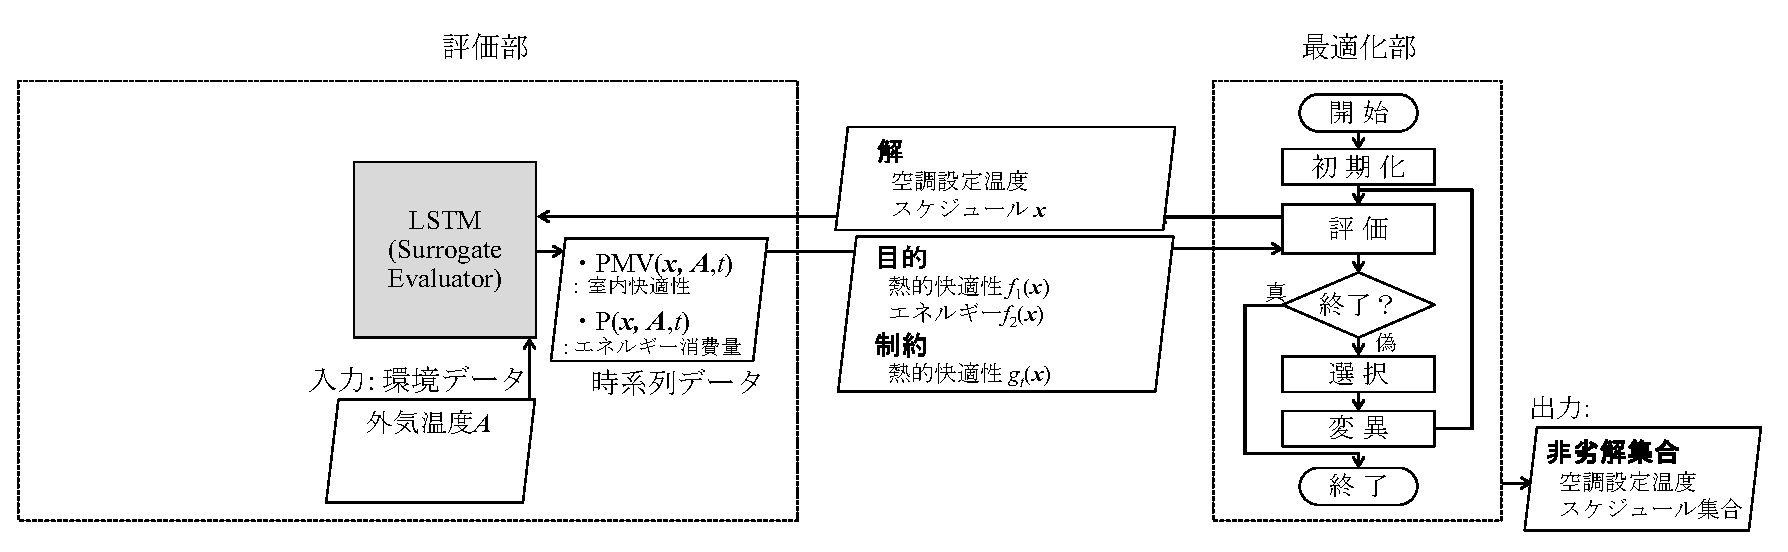
\includegraphics[width=1.1\linewidth]{fig/surrogate_system.eps}
  \end{center}
  \caption{サロゲート最適化システム}
  \label{fig::surrogate_system}
\end{figure*}

\section{サロゲート最適化における解評価}\label{sec::surrogate_model}
\subsection{サロゲート評価器の概要}
\secref{sec::sim_model}におけるEnergyPlusシミュレータの出力を低計算コストで模擬するサロゲート評価器を構築する.サロゲートモデルが代替するシミュレータ出力は時系列データであるため,本研究では,サロゲートモデルとしてRecurrent Neural Network (RNN)のひとつであるLSTM \cite{Gers00, Gers01}を用いた.LSTMは,過去の隠れ層の状態入力に加えて,内部にメモリセルと呼ばれる記憶部を導入し,入力・忘却・出力の3つのゲートによって過去の状態を保持して利用する.これにより,短期の記憶に加えて長期記憶を利用した時系列データの予測が可能であり,自然言語処理など時系列データを取り扱う分野で高い効果があることが知られている\cite{Sutskever14}.空調の快適性およびエネルギー消費量は,直近の時刻の値に影響されるほか,外気温に依存して変動するため周期性を持ち当日の最低気温や前日の最高気温などの影響を大きく受ける.そのため,長短期記憶を活用できるLSTMを採用することで,精度の高い予測が期待できる.本章の最適化システムでは,LSTMを隠れ層とする\figref{fig::surrogate_nn}に示す構成のニューラルネットワークを,室内快適性とエネルギー消費量の時系列データの予測に利用する.

\begin{figure*}[ht]
  \begin{center}
    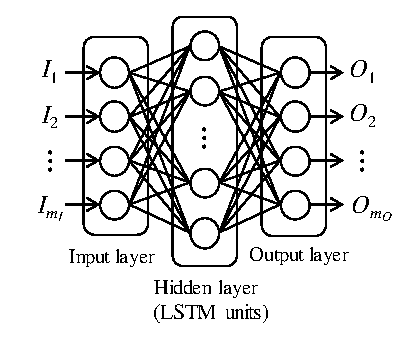
\includegraphics[width=0.65\linewidth]{fig/surrogate_nn.eps}
  \end{center}
  \caption{LSTMに基づくサロゲート評価器のネットワーク構成}
  \label{fig::surrogate_nn}
\end{figure*}

\subsection{サロゲート評価器のネットワーク構成}
\figref{fig::surrogate_nn}のネットワークにおいて,$I_i$ $(i=1, 2,\dotsc,m_{I})$と $O_j$ $(j=1, 2,\dotsc,m_{O})$はそれぞれ入力と出力値であり,$m_{I}$は入力層の入力値と入力ユニットの数で,$m_{O}$は出力層における出力値と出力ユニットの数である.入力と出力の間の隠れ層はLSTM層であり,LSTM層の全ユニットは入力層と出力層に全結合されている.LSTM層のユニット数は$m_{H}$である.

\begin{figure}[t]
  \begin{center}
    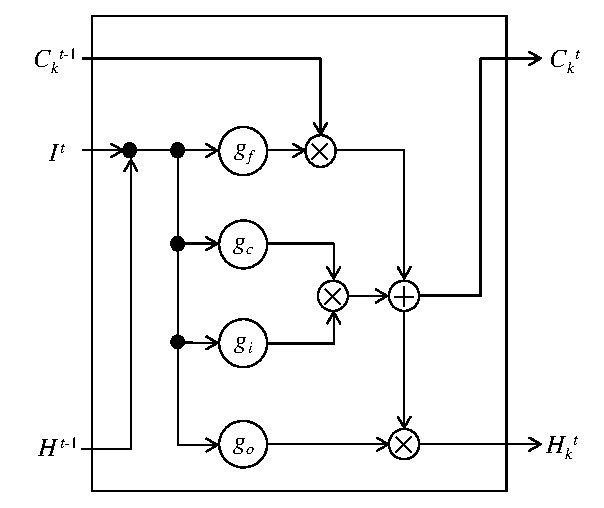
\includegraphics[width=0.5\linewidth]{fig/surrogate_lstm.eps}
  \end{center}
  \caption{サロゲート評価器のLSTMの1ユニットの構成}
  \label{fig::surrogate_lstm}
\end{figure}

\figref{fig::surrogate_lstm}は本研究で使用しているLSTMユニットの構造を示す\cite{Gers00}.この図は$k$番目のLSTM層を示す.ここで,$I^t$, $H_k^t$と$C_k^t$はそれぞれタイムステップ$t$におけるLSTM層の入力ベクトル,$k$番目のLSTM層の状態,$k$番目のLSTM層のメモリセル状態である.$g_f$は忘却ゲート,$g_c$はメモリセルゲート$g_{i}$は入力ゲートで,$g_{o}$は出力ゲートである.
タイムステップ$t$の$k$番目の各ゲートの出力値は以下の式で計算される.
\begin{align}
  O^{Gt}_k = f^G \left( \sum^{m_I}_{i = 1}{w^G_{ki} \cdot I^t_i} + \sum^{m_H}_{h = 1}{u^G_{kh} \cdot H^{t-1}_h} + \theta^G_k \right) \nonumber \\~~~~~~~(k=1,2,\dots,m_H)
\end{align}

ここで$G$はゲート種類($g_f$, $g_c$, $g_i$, $g_o$),$w$は入力$I^t$の重み係数,$u$はLSTMユニット$H^{t-1}$の前回状態の重み係数, $\theta$はバイアス項,$f^G$はゲート$G$の活性化関数である.$f^{g_c}$の活性化関数として双曲線正接関数を用いた.他のゲートにはシグモイド関数を活性化関数として用いた.メモリセル状態$C^t_k$は以下の式で計算される.
\begin{equation}
  C^t_k = O^{g_it}_k \cdot O^{g_c t}_k + O^{g_ft}_k \cdot C^{t-1}_k
\end{equation}
そして,$k$番目のLSTMユニットの状態$H^t_k$は以下の式で計算される.
\begin{equation}
  H^t_k = O^{g_ot}_k \cdot \tanh(C^t_k)
\end{equation}
出力層の各ユニットの出力値は以下の式で算出される.
\begin{equation}
  O_{j}  = f_{O} \left(\sum^{m_{H}}_{k=1} w_k \cdot H_k + \theta_{j} \right)~~(j=1, 2,\dotsc,m_{O}) \label{eq::fully_connected_output}
\end{equation}
ここで,$H_k$はLSTM層のk番目のユニットの出力,$w_k$はその重み係数,$\theta_{j}$は$j$番目の出力ユニットのバイアス項,そして$f_{O}$は出力層の活性化関数である.$f_{O}$の活性化関数には恒等関数を用いた.

\subsection{サロゲート評価器の入出力}
\figref{fig::surrogate_nn}に示したネットワークについて,入力としてタイムステップ$t$における空調設定温度$t_{set}(\vec{x},t)$を入力し,快適性レベル$TCFM(\vec{x}, \mathcal{A}, t)$とエネルギー消費量$ASEE(\vec{x}, \mathcal{A}, t)$の2つの時系列データを出力として得る.これらの出力値は気象条件の影響を受けるため,同様に外気温度と外気湿度も入力する.ここで\figref{fig::surrogate_nn}の入力はタイムステップ$t$のデータのみであり,\figref{fig::surrogate_nn}の出力はその結果のみであることに注意されたい.そのため,時系列の出力を得るためには,時系列の入力データを繰り返し\figref{fig::surrogate_nn}のネットワークに入力しなければならない.入出力を繰り返す間,\figref{fig::surrogate_nn}のLSTMユニットは以前のタイムステップの状態を保持して予測する.提案システムにおいて,入力値とユニットの数は$m_{I}=3$であり,$I_1$, $I_2$, $I_3$はそれぞれタイムステップ$t$における空調設定温度$t_{set}(\vec{x},t)$,外気温度$a_t$,外気湿度である.出力値とユニットの数$m_{o}=2$であり,$O_1$は室内快適性レベル$TCFM(\vec{x}, \mathcal{A}, t)$で,$O_2$はエネルギー消費量$ASEE(\vec{x}, \mathcal{A}, t)$である.

\begin{figure*}[ht]
  \begin{center}
    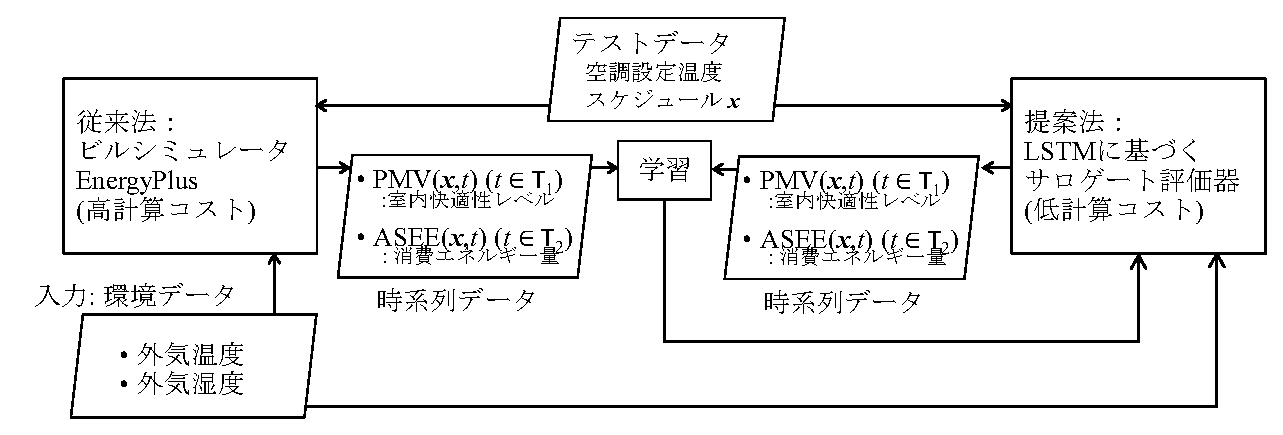
\includegraphics[width=1.1\linewidth]{fig/surrogate_learn_system.eps}
  \end{center}
  \caption{LSTMに基づくサロゲート評価器の学習}
  \label{fig::surrogate_learn_system}
\end{figure*}

\subsection{サロゲート評価器の学習}
本研究では,LSTMベースのサロゲート評価器を7日分の学習データで学習する.\figref{fig::surrogate_learn_system}に学習プロセスのフロー図を示す.学習用の入力データとして,空調設定温度を\Eqref{eq::sim_constraint_tset_diff}の制約を満たすようにランダムに生成し,対象期間の気象データから得た実際の外気温度・外気湿度と合わせて使用する.教師データには,EnergyPlusシミュレータに学習用入力データを入力し出力した結果を用いた.

\section{実験内容}
本章では,最初に提案するLSTMに基づくサロゲート評価器の精度を,同一の入力から得られた従来のEnergyPlusシミュレーションの出力とサロゲート評価器の出力との比較により確認する.次に,提案するサロゲート評価器を用いた空調設定温度スケジュール最適化システムによる探索を実行し,その結果を考察する.

\begin{table}[t]
  \begin{center}
    \caption{LSTMのパラメータ}
    \label{tab::surrogate_param_lstm}
    \begin{tabular}{c|cccc}
      \hline
      パラメータ                             & 値    \\
      \hline \hline
      ミニバッチサイズ                       & 200   \\
      学習回数                               & 2000  \\
      LSTM層のユニット数 $m_h$               & 250   \\
      最適化手法                             & Adam  \\
      学習率 $\alpha$                        & 0.001 \\
      勾配の移動平均の減衰率 $\beta_1$       & 0.9   \\
      勾配の二乗の移動平均の減衰率 $\beta_2$ & 0.999 \\
      \hline
    \end{tabular}
  \end{center}
\end{table}

\subsection{ビルエネルギーシミュレーションの設定}
気象データには2006年の拡張アメダスデータ\cite{Akasaka00}を用いた.一方,サロゲート評価器の学習のために,夏期2ヶ月間(7月1日~8月31日)を学習用の気象データとして用いた.室内温度設定の上下限値や室内の人の占有率,照明等の利用条件は\chapref{chap::sim}と同様とした.
最適化の対象日は夏期の代表日でありエネルギー消費量が大きくなる8月21日とした.

\subsection{サロゲート評価器の設定}\label{subsec::surrogate_setting}
\tabref{tab::surrogate_param_lstm}に提案システムで使用したLSTMネットワークを得るための学習パラメータを示す.予測誤差の評価のために,MSE(Mean Squared Error)を用いた.学習データは7月1日~8月25日を開始日とする7日間の時系列データをそれぞれ100個ずつ作成し,そのうち8割を訓練データとしてサロゲート評価器を訓練し,2割を検証データとして精度評価に用いた.入力と出力データの範囲は[0,1]に正規化した.
また,サロゲート評価器は7日間のデータを予測するため,最適化対象日である8月21日を7日目とする8月15日~8月21日のデータを用意して,最適化に利用した.入力データのうち7日目の空調設定温度を設計変数に応じて変更してサロゲート評価器による予測を行い,出力として得られた7日間の時系列データのうち7日目のデータを用いて目的関数計算を行った.
サロゲート評価器はPython言語によって実装し,Windows 10(64bit),Intel Core i7-3770K (3.5 GHz)CPUと16 GB RAMを持つPCで実行した.また,サロゲート評価器はWebサーバとし,最適化部からのリクエストとして設計変数を受領し,その設計変数に対する評価値をレスポンスとして返すようにした.従来のEnergyPlusシミュレータは,シミュレータ仕様の制約からファイルインターフェースによる設計変数と時系列データを授受していたが,ファイル入出力処理に時間がかかりオーバーヘッドが発生していた.これをパケット通信によるデータ授受とすることで高速化を図った.同一のPC上にサロゲート評価プロセス,サーバプロセス,最適化プロセスが複数存在していることから,解評価は並列化せず,1度に1つの解のみを評価することとした.

\begin{comment}

\begin{table}[t]
  \begin{center}
    \caption{OMOPSOのパラメータ}
    \label{tab::surrogate_param_omopso}
    \begin{tabular}{c|cccc}
      \hline
      パラメータ                             & 方法/値                \\
      \hline \hline
      ベース粒子群サイズ $|\mathcal{P}|$     & 35                     \\
      リーダー粒子群サイズ $|\mathcal{L}|$   & 100                    \\
      アーカイブ粒子群サイズ $|\mathcal{A}|$ & 制限なし               \\
      総世代数 $g^{max}$                     & 500                    \\
      設計変数の数 $n$                       & 20                     \\
      突然変異率 $p_m$                       & 1/$n$                  \\
      非一様突然変異の係数 $b$               & 5 \cite{Esquivel03}    \\
      重み $w$                               & [0.1, 0.5)の一様乱数   \\
      重み $c_1, c_2$                        & [$1.5, 2.0$)の一様乱数 \\
      $\epsilon$-dominanceの係数$\epsilon$   & 0.0075                 \\
      \hline
    \end{tabular}
  \end{center}
\end{table}

\end{comment}

\subsection{最適化部の設定}\label{subsec::surrogate_setting_omopso}
OMOPSOで用いるパラメータは\tabref{tab::sim_param_omopso}と同一とした.ただし,粒子群サイズは35個体とした.EnergyPlusシミュレータの実行プログラムとOMOPSOアルゴリズムは\secref{sec::sim_setting}同様Javaで実装し,計算は前項に記載したPCと同一のPCで実行した.

\section{実験結果と考察}\label{sec::surrogate_result}

\begin{table}[t]
  \begin{center}
    \caption{サロゲート評価器の検証データに対する予測誤差率(MAPE)}
    \label{tab::surrogate_predict}
    \small
    \begin{tabular}{c|c|c}
      \hline
      対象データ & 室内快適性(PMV) & エネルギー消費量 \\
      \hline \hline
      MAPE[\%]   & 0.305           & 1.25             \\
      \hline
    \end{tabular}
  \end{center}
\end{table}

\begin{figure}[t]
  \centering
  \subfigure[室内快適性(PMV)]{
    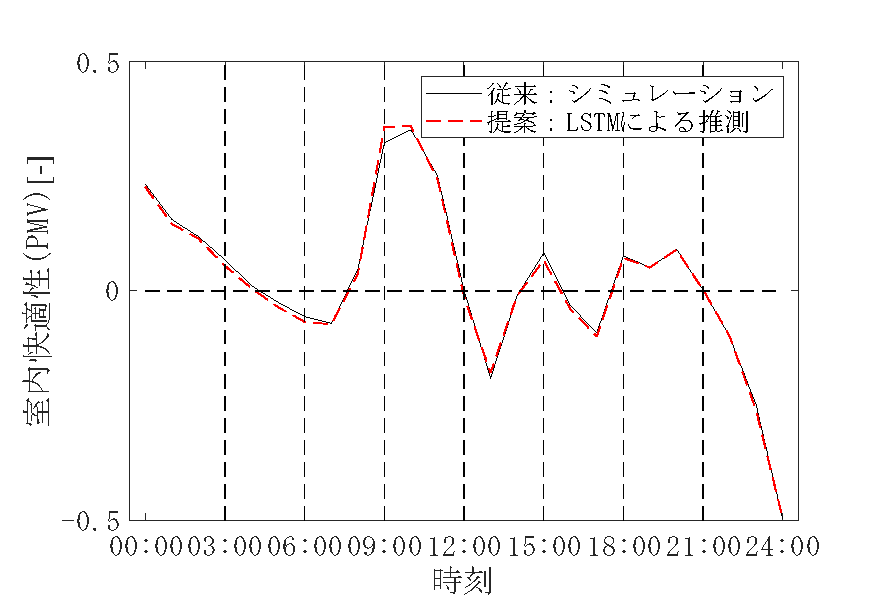
\includegraphics[width=0.7\textwidth,keepaspectratio=true]{fig/surrogate_predict_1.eps}
    \label{fig::surrogate_predict_pmv}
  }
  \subfigure[エネルギー消費量]{
    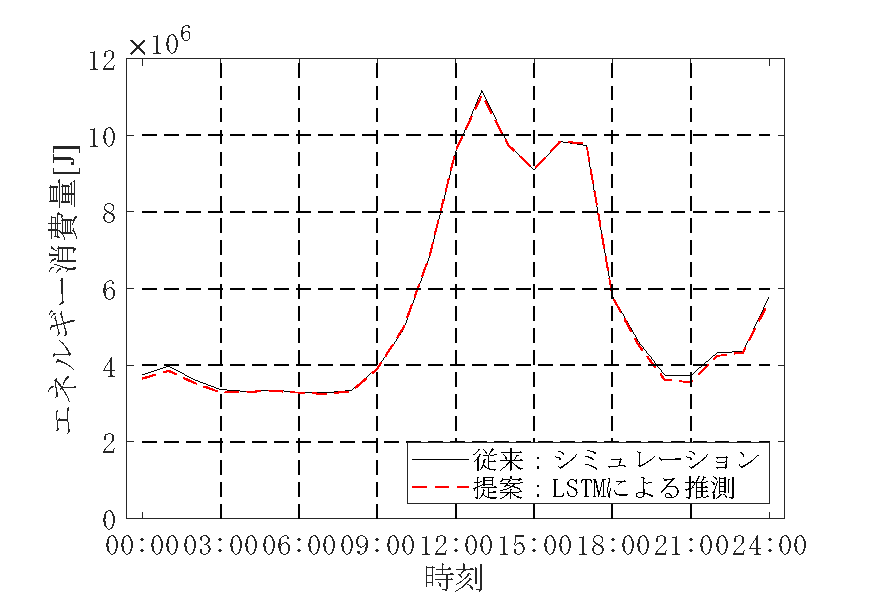
\includegraphics[width=0.7
      \textwidth,keepaspectratio=true]{fig/surrogate_predict_2.eps}
    \label{fig::surrogate_predict_power}
  }
  \caption{従来法であるEnergyPlusシミュレータと提案するサロゲート評価器の時系列データの出力結果}
  \label{fig::surrogate_predict}
\end{figure}

\subsection{提案するLSTMベースのサロゲート評価器の予測精度}
最初に,提案するLSTMベースサロゲート評価器の精度を確認する.LSTMベースサロゲート評価器を上述の学習データで学習し,サロゲート評価器の出力と真値との誤差を検証データを用いて確認した.誤差の評価には,平均絶対パーセント誤差(Mean Absolute Percentage Error, MAPE)を用いた.MAPEの定義は以下の通りである.

\begin{align}
  \label{eq::surrogate_error_rate}
  MAPE & = \frac{100}{n_{valid}} \sum^{n_{valid}}_{t=1} |\frac{V_{predict}(t)-V_{actual}(t)}{V_{actual}(t)}|
\end{align}

ここで$V_{actual}$はシミュレータの出力した時系列データの真値,$V_{predict}$はLSTMベースのサロゲート評価器が出力した推測値である.全ての検証データを系列として並べて,MAPEを算出した.検証データの個数$n_{valid}=184,800$である.室内快適性(PMV)およびエネルギー消費量それぞれについてMAPEを算出したところ,結果は\tabref{tab::surrogate_predict}のとおりとなった.室内快適性の誤差率は0.305\%,エネルギー消費量の誤差率は1.25\%であり,提案したサロゲート評価器は2つの時系列データを十分に小さい誤差で推測可能であるということがわかる.\figref{fig::surrogate_predict}に,EnergyPlusシミュレーションとサロゲート評価器で得られた室内快適性とエネルギー消費量の2つの時系列データの1日の検証データの例を示す.提案するサロゲート評価器から得られた値はシミュレータの結果の動きを予測できていることがわかる.これらの結果から,提案するLSTMに基づくサロゲート評価器はEnergyPlusシミュレータの代替として妥当であることが確認できた.

\begin{figure}[ht]
  \begin{center}
    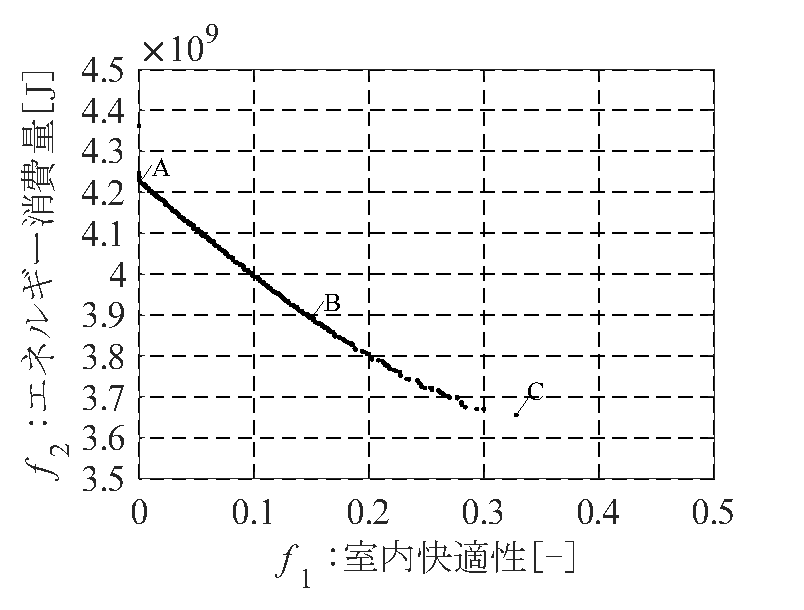
\includegraphics[width=0.8\linewidth]{fig/surrogate_result_pareto.eps}
  \end{center}
  \caption{サロゲート最適化の結果}
  \label{fig::surrogate_result_pareto}
\end{figure}

\subsection{多目的最適化によって得られたスケジュール}
\figref{fig::surrogate_result_pareto}に提案するLSTMに基づくサロゲート評価器を用いて得た最終世代の全ての解(空調スケジュール)を示す.横軸と縦軸はそれぞれ最小化する空調システムの室内快適性指標とエネルギー消費量を示す.各点は空調設定温度スケジュールの目的関数値を示す.今回は143個のスケジュールが獲得できた.この結果から,提案システムは対象ビルの空調システムにおける室内快適性とエネルギー消費量のトレードオフを近似する解が得られることがわかる.小さい$f_1$の値を持つ快適な温度設定スケジュールは空調システムの運転にあたりエネルギー消費量$f_2$を妥協し,$f_2$の小さい省エネな空調設定温度スケジュールはビルのオフィスワーカーの環境快適性$f_1$を犠牲にする.

次に,提案システムによって得られたスケジュールの時系列データを確認する.\figref{fig::surrogate_result_pareto}の3つのスケジュールA, B, Cについて,それぞれの時系列の空調設定温度,室内快適性PMV指標,エネルギー消費量を\figref{fig::surrogate_result_schedule}に示す.室内快適性とエネルギー消費量の図には,提案するLSTMに基づくサロゲート評価器とEnergyPlusシミュレーションの双方の出力を描画した.

結果として,室内快適性レベルは$[-0.5, 0.5]$の中に収まっており,最低快適性レベルに関する制約\Eqref{eq::math_constraint_pmv}を満たす実行可能なスケジュールが得られている.加えて,2つの連続した時刻間の温度設定変更幅は2.0 [$^\circ$C]以内であり,設定温度変更幅の\Eqref{eq::sim_constraint_tset_diff}を満たす実行可能なスケジュールが得られていることがわかる.

\figref{fig::surrogate_result_schedule}に示すとおり,各スケジュールA~Cでは,サロゲート評価器とEnergyPlusシミュレーションの2つの出力の差は小さい.これは,提案するサロゲート評価器が探索したスケジュールに対して高精度に予測できるためであり,提案するLSTMベースのサロゲート評価器がEnergyPlusシミュレーションの代替としてうまく機能している結果であるといえる.\red{一方で,1日のうち5:00~7:00の時間帯に,サロゲート評価器とEnergyPlusシミュレーションの誤差がやや大きくなる傾向がある.しかし,この時間帯はビル内の在室者数が少なく,エネルギー消費量も比較的大きくないことから,誤差の目的関数評価への影響は小さく,問題がない程度であると考える.}
\begin{comment}
一方で,スケジュールBとCではEnergyPlusシミュレータの出力とサロゲート評価器の出力の差が大きくなってしまった.これは,LSTMの学習データに,スケジュールBやCと同様のスケジュールが十分な数存在せず,学習が不足しているためであると考える.スケジュールBやCは快適性の制約\Eqref{eq::math_constraint_pmv}の境界値である$PMV=0.5$に近い$PMV$値を持つスケジュールであるが,このようなスケジュールは\subsecref{subsec::surrogate_setting}で述べた手法でランダム生成した学習データに十分な量含まれていない.そのため,サロゲート評価器は学習の際に予想していなかったデータの推定をするという状況となっており,予測精度が低下している.BやCのようなスケジュールにも対応するためには,室内快適性制約\Eqref{eq::math_constraint_pmv}の境界値に近い値を持つ解を学習データに含めること,もしくは,最適化プロセスの途中で得られた解EnergyPlusシミュレーション評価器で評価してLSTMサロゲート評価器の学習と更新を並行して進めることが必要であると考える.これらの手法により,スケジュールBやCのような解に対してもサロゲート評価器の精度の向上と誤差の低減が期待できる.
\end{comment}
実験結果から,提案するLSTMベースサロゲート評価器は実行可能で実用的な空調設定温度スケジュールを獲得するのに有用であるといえる.

\begin{figure*}[htbp]
  \begin{center}
    \begin{minipage}{0.45\textwidth}
      \begin{center}
        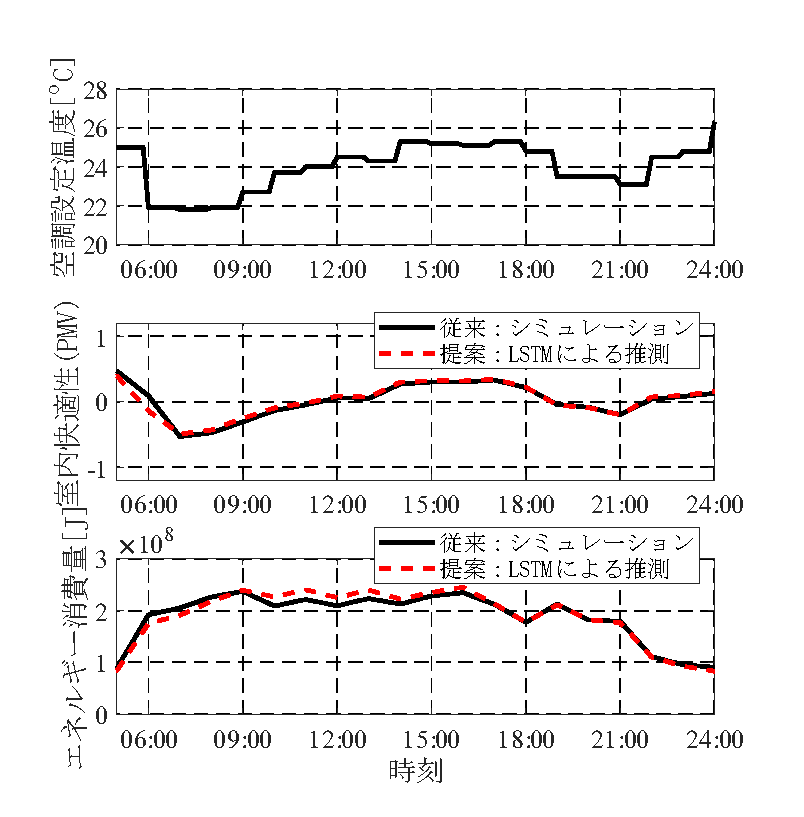
\includegraphics[width=1\textwidth,keepaspectratio=true]{fig/surrogate_result_schedule_a.eps}\\\vspace{-5mm}{\small スケジュールA (最も快適な解)}
      \end{center}
    \end{minipage}
    \\
    \begin{minipage}{0.45\textwidth}
      \begin{center}
        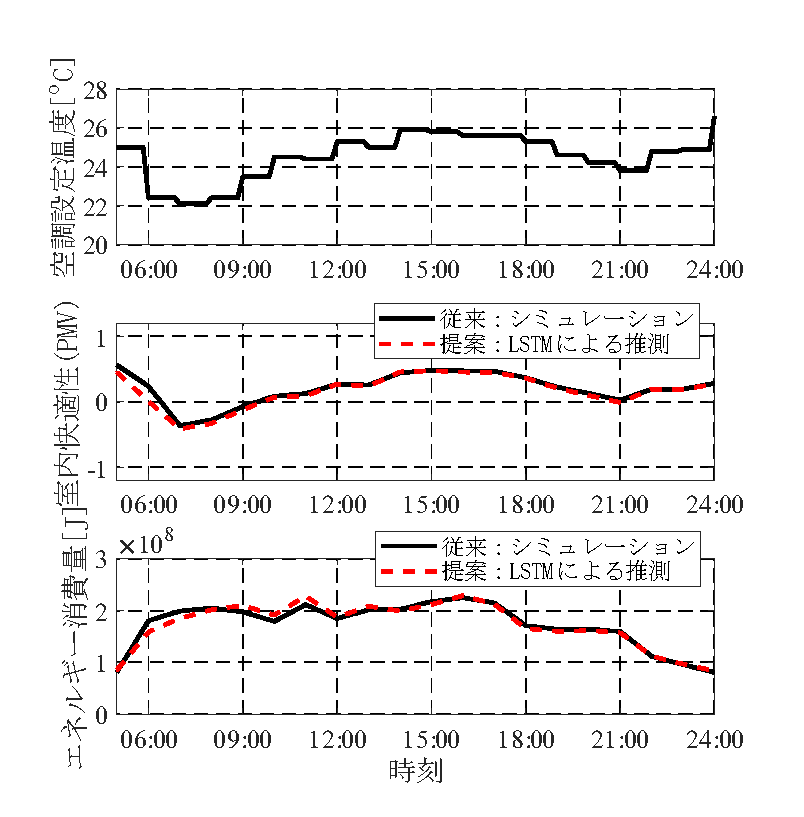
\includegraphics[width=1\textwidth,keepaspectratio=true]{fig/surrogate_result_schedule_b.eps}\\\vspace{-5mm}{\small スケジュール B (中間の解)}
      \end{center}
    \end{minipage}
    \\
    \begin{minipage}{0.45\textwidth}
      \begin{center}
        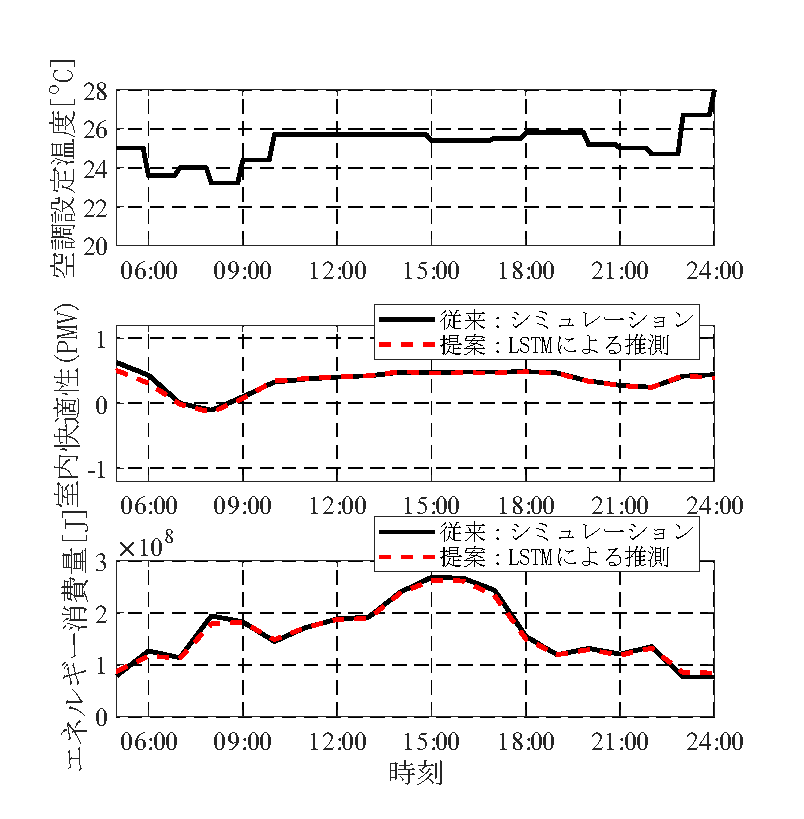
\includegraphics[width=1\textwidth,keepaspectratio=true]{fig/surrogate_result_schedule_c.eps}\\\vspace{-5mm}
        {\small スケジュール C (最も省エネな解)}
      \end{center}
    \end{minipage}
    \vspace{-1mm}
    \caption{OMOPSOによって得られた空調設定温度スケジュールの時系列データの例}
    \label{fig::surrogate_result_schedule}
  \end{center}
\end{figure*}


\subsection{計算時間}
\tabref{tab::surrogate_result_time}に1つの解の評価時間と,最適化の全体の計算時間を示す.ここで,従来システムと提案システムを同じ評価回数で比較するために,従来システムの結果として個体数を本章の設定である35個体とした場合の計算時間を用いている.提案したLSTMに基づくサロゲート評価器の結果は,最適化を20回試行した平均値である.この結果から,1つのスケジュールの評価には,提案するサロゲート評価器は従来のEnergyPlusシミュレーションに対しておおよそ310倍高速であることがわかる.加えて,提案システムの全体の評価時間は0.493時間であり,これは従来手法の1/47である.したがって,提案システムは空調設定スケジュールの進化的最適化を高速化できるといえる.
提案するサロゲート評価器により評価を高速化することにより,進化計算においてより多数の個体や世代での評価が可能となる.そのため,従来システムと同等の時間でも目的関数値が改善されたより良好なスケジュールを獲得することが期待できる.また,1日の空調設定スケジュールを獲得するために,従来システムでは概ね1日必要とするため,1日前に計算を開始する必要があった.外気温度・外気湿度などの気象予報の精度は時間が直近になるほど高精度となり最適化結果の改善につながる.そのため,空調設定スケジュールを用いた空調運転のなるべく直前の予報値を利用できることが望ましいが,従来手法では運転開始の1日前と精度の低い予報値しか利用することができなかった.提案するサロゲート評価器によるスケジュール評価の高速化は最適化の高速化だけでなく,信頼性の高い気象予報データを使用することによるスケジュールの品質改善にも寄与するといえる.
さらに,提案システムでは,使用したPCのスレッド数の制約から解評価を並列化しなかった.より多数のスレッドで計算可能なPCの採用により解評価を並列化できれば,さらに計算時間を短縮することが可能と考える.

\begin{table}[t]
  {\footnotesize
    \begin{center}
      \caption{計算時間の比較}
      \label{tab::surrogate_result_time}
      \begin{tabular}{c|cccc}
        \hline
                                 & 従来システム                 & 提案システム                   \\
                                 & (EnergyPlusシミュレーション) & (LSTMに基づくサロゲート評価器) \\
        \hline \hline
        1つの解の平均評価時間    & 37.3 [秒]                    & 0.120 [秒]                     \\
        最適化全体にかかった時間 & 23.4 [時間]                  & 0.493[時間]                    \\
        \hline
      \end{tabular}
    \end{center}
  }
\end{table}

\section{多目的粒子群最適化アルゴリズム改善案の検証}
\subsection{目的}

本章では,LSTMに基づくサロゲート評価器を用いた進化的空調設定スケジュールの多目的最適化の高速化手法を提案した.本手法により最適化時間を従来用いていたEnergyPlusシミュレータの1/47とすることができ,高速にパレート解集合を獲得可能となった.しかし,一度の最適化には依然として30分近い時間がかかっている.この時間をさらに短縮できるとより信頼性の高い気象データの利用やビル管理者の利便性向上につながる.今回用いた評価回数は17,500回(35個体×500世代)であるが,より少ない評価回数でも同様のパレート解集合が獲得できることが望ましい.また,少ない評価回数で同様のパレート解集合が獲得できた場合,評価回数を今回と同程度まで増やすことで,同じ時間でさらに良好な解が探索できる可能性がある.そこで,この空調設定スケジュール最適化問題に対して,より少ない評価回数でも良好な解を探索可能な進化計算アルゴリズムが望まれる.
\secref{sec::sim_valid}で述べたように,従来のEnergyPlusシミュレータによる評価では1度の最適化プロセスに長時間かかるため,良好なアルゴリズムやそのパラメータを試行錯誤し,その性能の検証を行うことは困難であった.しかし,本章で提案したサロゲート評価器による高速化により,短い時間での最適化とその複数回の試行が現実的な時間で可能となった.
本節では,提案したサロゲート評価器を用い,複数の多目的進化計算法によって得られる解集合の性能比較を行う.また,より少ない評価回数で良好な解を探索可能な手法としてOMOPSOを改良した手法を提案し,その性能を検証する.

\subsection{方法}
\subsecref{subsec::sim_algo}と同じく,4種類の多目的進化計算法OMOPSO,NSGA-II,NSGA-III,MOEA/D-DEを比較する.加えて,OMOPSOの探索性能を改良した手法としてDOMOPSOを提案する.

\subsubsection{DOMOPSO(Directional OMOPSO)}
OMOPSOの特徴は,\subsecref{subsec::OMOPSO}で述べたように,アーカイブを持つこと,非一様な突然変異操作を持つこと,アーカイブから抽出されたリーダー粒子群からバイナリトーナメントでgBestを選択することである.特に,PSOの探索においてgBestは解集合全体の方向性を目標づける重要な役割を持つことから,本研究では,アルゴリズム改良のポイントとしてOMOPSOにおけるgBestの選択方法に着目する.OMOPSOでは,飛翔対象の粒子ごとにリーダー粒子群からgBestをバイナリトーナメントで選択する.この手法は,解の多様性の獲得を大きな目的とする多目的最適化において有効な働きをするが,一方で解の収束性に対しては有効に働く場合とそうでない場合がある.\figref{fig::surrogate_algorithm}を使って,パレートフロント近くに到達していない段階において,選択されるgBestによっては良好な解が得られにくいことを示す.\figref{fig::surrogate_algorithm_omopso}に青で示した飛翔対象粒子に対して,リーダー粒子群の中から(1)がgBestとして選択された場合,飛翔対象粒子はパレートフロント方向に飛翔することとなり,パレートフロントへの収束を進めることができる.一方で(2)のようなgBestが選択されると,gBestへの方向はパレートフロントに近づくことにはならず,良好な解の発見に寄与しない.このようなgBestの選択が多いと,パレート解集合の収束性の低下を招く恐れがある.そこで,本節では,gBestの選択方法を改良した新たなOMOPSOアルゴリズムを提案する.\figref{fig::surrogate_algorithm_domopso}のように,gBestの選択時に,リーダー粒子群のうち飛翔対象の粒子を優越している解の中からgBestをバイナリトーナメントで選択することで,探索空間における飛翔対象粒子が目指すべきパレートフロントとはかけ離れた方向への探索を抑制することが可能となる.この手法によって,OMOPSOの探索中の収束性の向上を図る.
本手法を,gBestの選択に方向性をもたせるという意味合いでDirectional OMOPSO(DOMOPSO)と呼称する.
DOMOPSOは,\subsecref{subsec::OMOPSO}で述べたOMOPSOのアルゴリズムのうちStep 4を改良することによって実現できる.改良したDOMOPSOのアルゴリズムのStep 4を以下に示す.

\begin{description} \label{algo::DOMOPSO}
  \setlength{\listparindent}{0pt}   %5. 最初のインデント
  \setlength{\itemsep}{0pt}      %2. ブロック間の余白    
  \item[Step 4:]
        各粒子$\vec{x}^g \in \mathcal{P}$の速度と位置を\Eqref{eq::theory_pso_velocity}, \eqref{eq::theory_pso_position}で更新する.
        ただし,$\vec{x}_{gbest}$は,$\mathcal{L}$のうち$\vec{x}^g$を$\epsilon$優越するリーダー粒子の中からバイナリトーナメント選択で選択された粒子の位置とする.$\mathcal{L}$に$\vec{x}^g$を$\epsilon$優越するリーダー粒子が存在しない場合,$\vec{x}_{gbest}$は$\mathcal{L}$全体の中からバイナリトーナメント選択で選択された粒子の位置とする.

        更新した$\vec{x}^{g+1}$の各要素が,[$x^{min}, x^{max}$]の範囲を超過した場合,境界値まで引き戻し,さらに速度$\vec{v}^{g+1}$を$-1$倍する修復操作を施す.
\end{description}

\begin{figure}[htbp]
  \centering
  \subfigure[従来:OMOPSO]{
    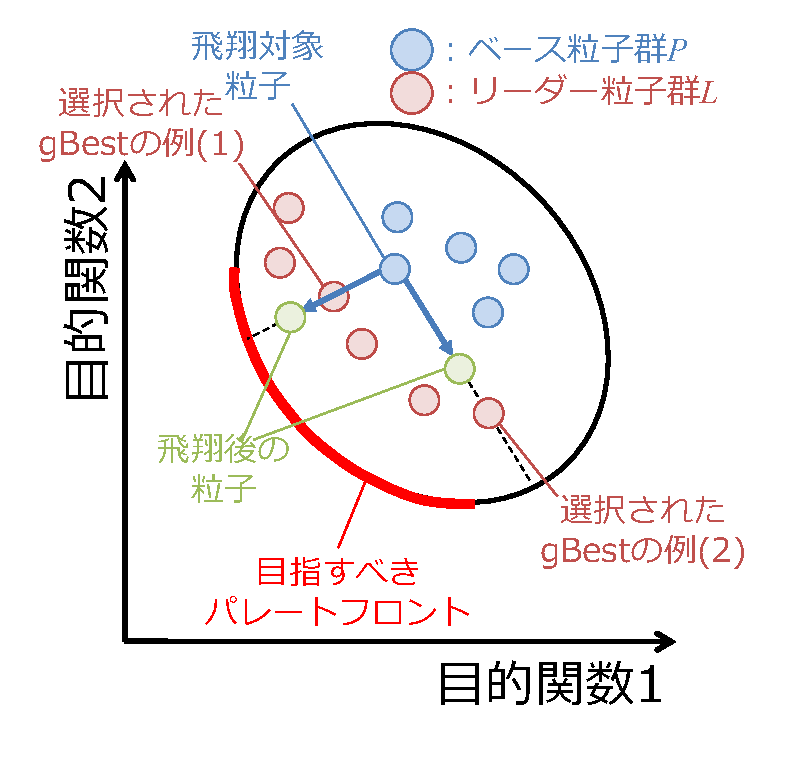
\includegraphics[width=0.7\textwidth,keepaspectratio=true]{fig/surrogate_algorithm_omopso.eps}
    \label{fig::surrogate_algorithm_omopso}
  }
  \subfigure[提案:DOMOPSO]{
    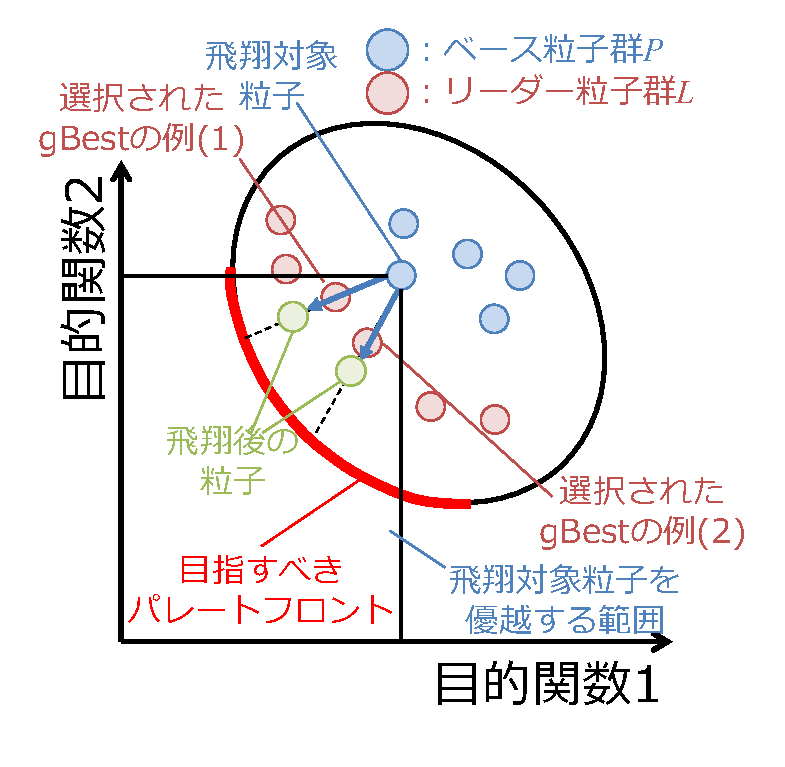
\includegraphics[width=0.7
      \textwidth,keepaspectratio=true]{fig/surrogate_algorithm_domopso.eps}
    \label{fig::surrogate_algorithm_domopso}
  }
  \caption{OMOPSOと改良手法であるDOMOPSOにおけるgBestの選択方法とその効果}
  \label{fig::surrogate_algorithm}
\end{figure}

\subsubsection{探索パラメータ}
OMOPSO, NSGA-II, NSGA-III, MOEA/D-DEに,提案するDOMOPSOを加えた5種類のアルゴリズムを用いて,サロゲートモデルによる評価を用いた空調設定スケジュール最適化問題のスケジュールを探索した.解集団サイズは35,総世代数を500とした.OMOPSOおよびDOMOPSOのパラメータは\subsecref{subsec::surrogate_setting_omopso}と同一した.また,NSGA-IIとNSGA-IIIのパラメータは\tabref{tab::sim_param_nsga},MOEA/D-DEのパラメータは\tabref{tab::sim_param_moead}と同一とした.それぞれのアルゴリズムについて初期値のシードを変更して21回の試行を行った.
% 図に上下の分散を表すバーは必要か?

\begin{figure}[htbp]
  \begin{center}
    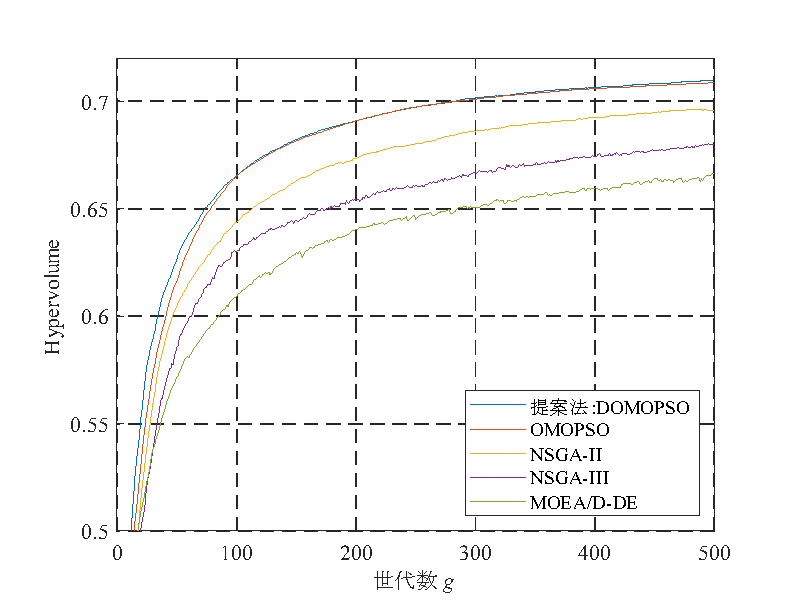
\includegraphics[width=0.7\linewidth]{fig/surrogate_result_algorithm_HV.eps}
  \end{center}
  \caption{5つの多目的進化計算法による探索性能(Hypervolume値)の世代推移}
  \label{fig::surrogate_result_algorithm_HV}
\end{figure}
\subsection{結果}
5種類のアルゴリズムそれぞれに対して,各世代で獲得された解のHypervolume(HV)を算出し,その各試行の平均値を求めて\figref{fig::surrogate_result_algorithm_HV}に示した.HVの算出条件は\subsecref{subsec::sim_algo}と同様とした.\figref{fig::surrogate_result_algorithm_HV}のうちまず提案法以外の手法を比較すると,OMOPSOが全世代にわたって最もよいHV値を示しており,次いでNSGA-II,MOEA/D-DEであった.NSGA-IIIは,本問題のような2目的で制約を持つ問題に対して良好な結果を示さないことがわかった.
次に,提案したDOMOPSOの性能を他の手法と比較する.DOMOPSOは8世代目まではOMOPSOと同程度のHV値を示しているが,以降の世代ではOMOPSOよりも高いHV値となった.リーダーアーカイブ$\mathcal{L}$に飛翔対象粒子を優越するような良好な解が格納されるまではDOMOPSOで採用した工夫の効果が現れにくいが,リーダーアーカイブ$\mathcal{L}$に良好な解が蓄積され始めるとDOMOPSOで採用した工夫によって良好な解を発見する割合が高くなり,OMOPSOよりも早期に良好な解集合に到達したものと考える.DOMOPSOのHV値をOMOPSOと比較すると,OMOPSOの500世代目のHV値は,DOMOPSOでは467世代目に到達している.そのため,DOMOPSOはOMOPSOが500世代かけて獲得する解集合と同程度のHV値の解集合を獲得するために,OMOPSOの約93.4\%程度の評価回数があればよく,従来法よりも6.6\%短い計算時間でパレート解集合が獲得できることになる.

\begin{figure}[htbp]
  \begin{center}
    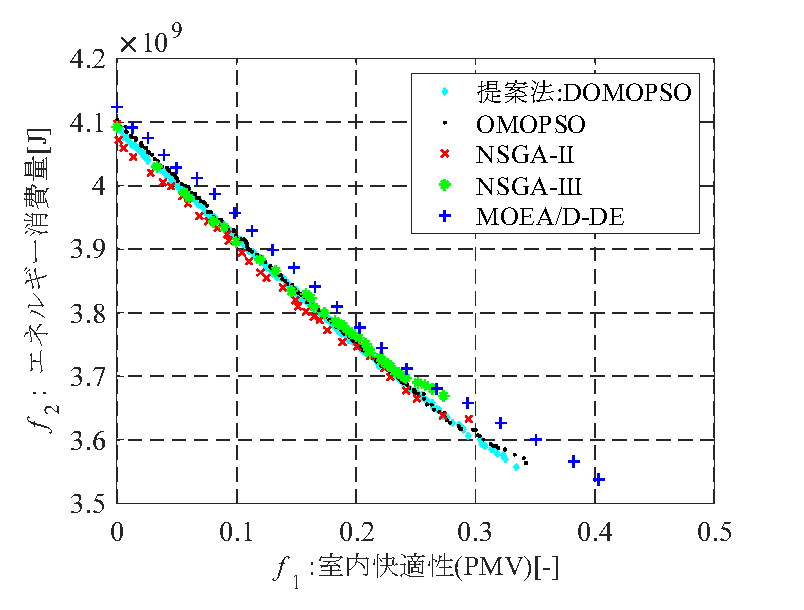
\includegraphics[width=0.7\linewidth]{fig/surrogate_result_pareto_algorithm.eps}
  \end{center}
  \caption{5つの多目的進化計算法による最終世代のパレート解集合(第1試行)}
  \label{fig::surrogate_result_pareto_algorithm}
\end{figure}

続いて,5種類のアルゴリズムの1回目の試行における最終世代の解集合を目的関数空間にプロットした結果を\figref{fig::surrogate_result_pareto_algorithm}に示す.この結果において,黒の点がOMOPSO,赤の×がNSGA-II,緑の*がNSGA-III,青の+がMOEA/D-DE,水色の◇が提案したDOMOPSOの結果である.結果の傾向は,\figref{fig::sim_result_pareto_multi}と似通っており,NSGA-II,NSGA-IIIは獲得された解集合の分布が狭いが,パレートフロントへの収束性の高い結果が得られている.MOEA/D-DEは目的関数空間に広域に分布するが,他の方法と比較してパレートフロントに対する収束性が低い.OMOPSOは,MOEA/D-DEの次に広い範囲に解集合が分布しており,かつパレートフロントへの収束性も高い良好な結果を得られている.提案したDOMOPSOは,通常のOMOPSOに対して,快適性に関する第一目的関数$f_1 \leq 0.1$と$f_1 \geq 0.3$の端の範囲で,さらにパレートフロントへの収束性が高く良好なパレート解集合を獲得できている.\red{特に$f_1 \geq 0.3$の範囲は,制約条件である$|f_1|>0.5$に近く実行可能な解の探索が困難な領域であるが,これらの領域でも提案したDOMOPSOはOMOPSOの解を優越する良好な解を獲得できており,探索性能が向上できていることが分かる.}これらの結果から,提案したDOMOPSOは,空調設定スケジュールの多目的最適化問題に対してOMOPSO,NSGA-II,NSGA-III,MOEA/D-DEよりも少ない評価回数で良好なスケジュールを獲得できるアルゴリズムであるといえる.

\section{サロゲートモデルを用いたロバスト最適化の検証}
\subsection{目的}
本章では,LSTMに基づくサロゲート評価器を用いることで,快適性とエネルギー消費量の2目的の進化的空調設定スケジュールの多目的最適化を高速化する手法を提案した.本手法で用いたLSTMに基づくサロゲート評価器では,外気温度・外気湿度および設計変数である空調設定温度を入力することで,時系列の室内快適性とエネルギー消費量を出力することができる.そこで,外気温度に気温予報誤差を加味した値を入力することで,5章で述べたロバスト最適化における気温予報誤差がある場合のロバストネスの評価が可能である.ロバスト最適化では,予報誤差のない場合の快適性・エネルギー消費量の評価に加え,ロバストネスの評価のために3回のEnergyPlusシミュレータの計算を実行する必要があり,最適化時間がかかる.そのため,ロバスト最適化においてもサロゲートモデルの使用による高速化が期待できる.
本節では,提案したサロゲート評価器を用い,ロバスト最適化による外気温予報誤差にロバストな空調設定温度スケジュールの探索を行う.獲得されたスケジュール集合をシミュレータと比較するとともに,最適化時間を高速化する効果について検証する.

\subsection{方法}
\chapref{chap::robust}で設計した気温予報誤差を含む外気温を,本章で提案したサロゲート評価器に入力しすることで,ロバストネスを評価する目的関数である\Eqref{eq::robust_objective3}, \eqref{eq::robust_objective4}を計算可能とする.
OMOPSOによって,サロゲート評価器による評価値を用いて,気温予報誤差を考慮せずに2つの目的関数値$f_1$, $f_2$を最適化した結果と,気温予報誤差を考慮して4つの目的関数$f_1$, $f_2$, $f_3$, $f_4$を最適化した結果を比較する.
サロゲートモデルは\subsecref{subsec::surrogate_setting}で述べたとおりPython言語によるWebサーバとして実装した.ロバスト最適化において必要な3回のシミュレーション(気温予報誤差が無い場合,上方気温予報誤差が発生した場合,下方気温予報誤差が発生した場合)をそれぞれ別のWebサーバとして同一マシン上で動作させることで,目的関数評価を並列化し最適化時間の高速化を図った.

\subsection{結果}
\subsubsection{多目的最適化によって獲得されたスケジュール}
\figref{fig::surrogate_result_pareto_robust}(a)に,サロゲート評価器を用い,ロバスト性を考慮せず目的関数値$f_1$, $f_2$を最適化した結果とロバスト性を考慮して目的関数$f_1$, $f_2$, $f_3$, $f_4$を最適化した結果を$f_1-f_2$目的関数空間上にプロットした結果を示す.
赤の丸が$f_1$, $f_2$のみを考慮して最適化した結果,黒の点が$f_3$, $f_4$も考慮した結果である.$f_1$, $f_2$がそれぞれ小さいほど室内快適性レベル・エネルギー消費量が少なく良好なスケジュールであることを示す.結果から,提案システムによって得られた結果はそれぞれ0.5未満であり,\Eqref{eq::math_constraint_violation_pmv}を満たして実行可能である.シミュレーションを用いたロバスト最適化による結果\figref{fig::robust_result_pareto}(a)と同様に,4目的の場合は$f_1$, $f_2$以外にロバスト性$f_3$, $f_4$という別の目的関数も考慮するため,2目的で最適化したほうが$f_1$, $f_2$においては良い目的関数値を示す解を獲得できる傾向がある.一方で4目的で最適化した結果は$f_1$, $f_2$においては悪い目的関数値を示す解も含んだ目的関数空間の広域に分布する解集合が得られることがわかる.同様にして獲得したスケジュールを$f_3$, $f_4$目的関数空間にプロットした結果を\figref{fig::surrogate_result_pareto_robust}(b)に示す.結果から,$f_3$, $f_4$を考慮した黒の点は,ロバスト性を考慮していない赤の点と同じか,それよりも値が小さいロバストな解を含む.シミュレーションを用いたロバスト最適化の結果\figref{fig::robust_result_pareto}(b)と比較すると,ロバスト性を考慮した4目的最適化の結果がロバスト性を考慮していない2目的最適化よりも小さい解を含む点は類似しているが,一方で解の分布形状の差は大きいことがわかる.

\begin{figure}[htbp]
  \begin{center}
    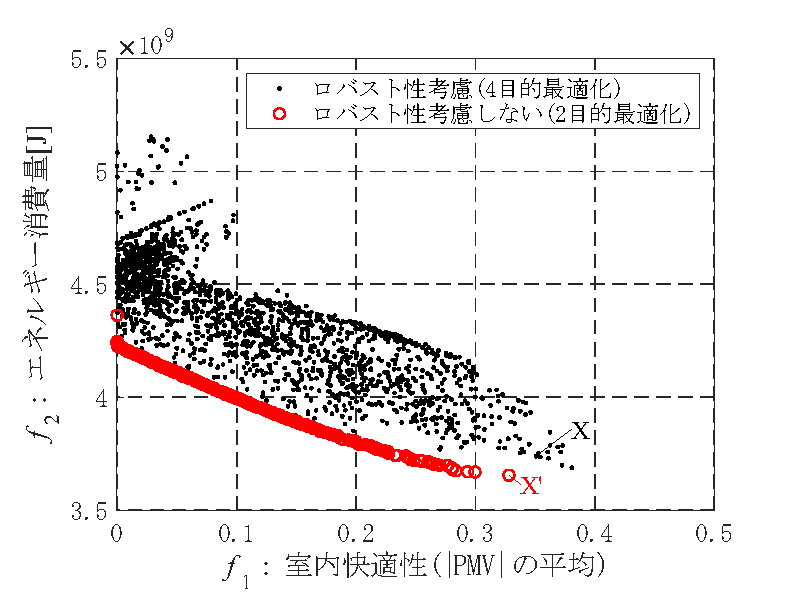
\includegraphics[width=0.7\columnwidth,keepaspectratio=true]{fig/surrogate_result_pareto_robust_f1f2.eps}\\
    {(a) $f_1$-$f_2$目的関数空間}
  \end{center}
  \begin{center}
    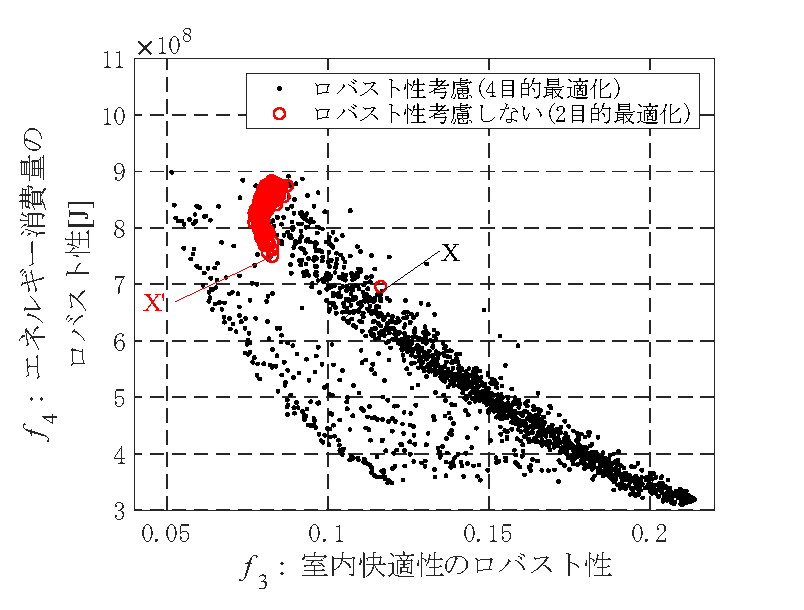
\includegraphics[width=0.7\columnwidth,keepaspectratio=true]{fig/surrogate_result_pareto_robust_f3f4.eps}\\
    {(b) $f_3$-$f_4$目的関数空間}
  \end{center}
  \caption{ロバスト最適化の結果}
  \label{fig::surrogate_result_pareto_robust}
\end{figure}

% スケジュールの描画と考察
サロゲート評価器を用いたロバスト最適化によって獲得したスケジュールのうち,\figref{fig::surrogate_result_pareto_robust}に示すように,$f_1$, $f_2$目的関数空間で近い値を持ち,かつ$f_3$, $f_4$目的関数空間で離れた値となる2つの解 X, X'を抽出し,それぞれの時系列のスケジュールを\figref{fig::surrogate_result_schedule_robust}に示す.これら2つの解は,$f_1$, $f_2$では近い目的関数値を持つが,解Xは$f_3$が小さく快適性に対してロバストであり,解X'は$f_4$が小さくエネルギー消費量がロバストであるという特徴の違いがある.\figref{fig::surrogate_result_schedule_robust}を見るとわかる通り,スケジュール X'は室内快適性は外気温予報誤差がある場合に,誤差が無い場合との差が大きいのに対して,スケジュール Xはその差が小さく抑制されている.一方で,Xはエネルギー消費量は外気温予報誤差がある場合とない場合の差が大きいが,X'はその差が小さくロバストである.
ロバスト性を考慮しない2目的最適化では,Xのような室内快適性についてロバストなスケジュールしか選択の余地がないが,ロバスト性を考慮した4目的最適化で獲得したスケジュールには,Xのような快適性のロバスト性が高いスケジュールだけでなく,X'のようなエネルギー消費量のロバスト性の高い解も選択することが可能である.さらに,室内快適性$f_3$, エネルギー消費量$f_4$いずれのロバスト性も向上することも可能である.このように,サロゲート評価器を用いたロバスト最適化が,\chapref{chap::robust}で述べたシミュレーションを用いたロバスト最適化と同様により多様な解を獲得することができ,意思決定者であるビル管理者に対して多様な選択肢を提供できる有用な手法であることが示された.

\begin{figure*}[htbp]
  \begin{center}
    \begin{minipage}{0.7\textwidth}
      \begin{center}
        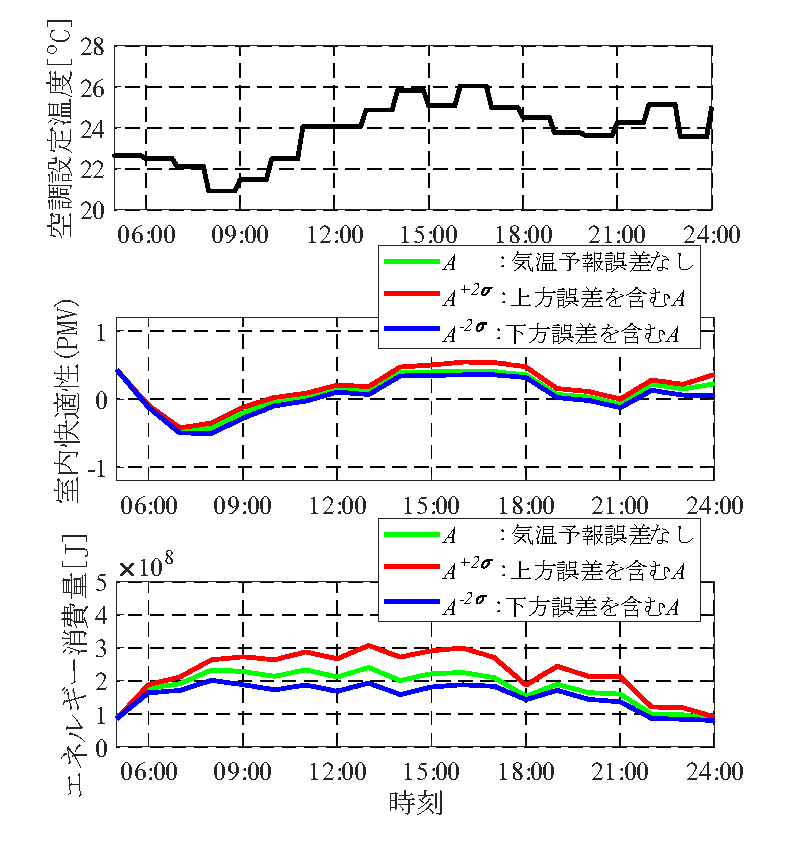
\includegraphics[width=1\textwidth,keepaspectratio=true]{fig/surrogate_result_schedule_robust_2obj.eps}\\\vspace{-5mm}{\small スケジュール X (ロバスト性を考慮しない2目的最適化で得た解)}
      \end{center}
    \end{minipage}
    \\
    \begin{minipage}{0.7\textwidth}
      \begin{center}
        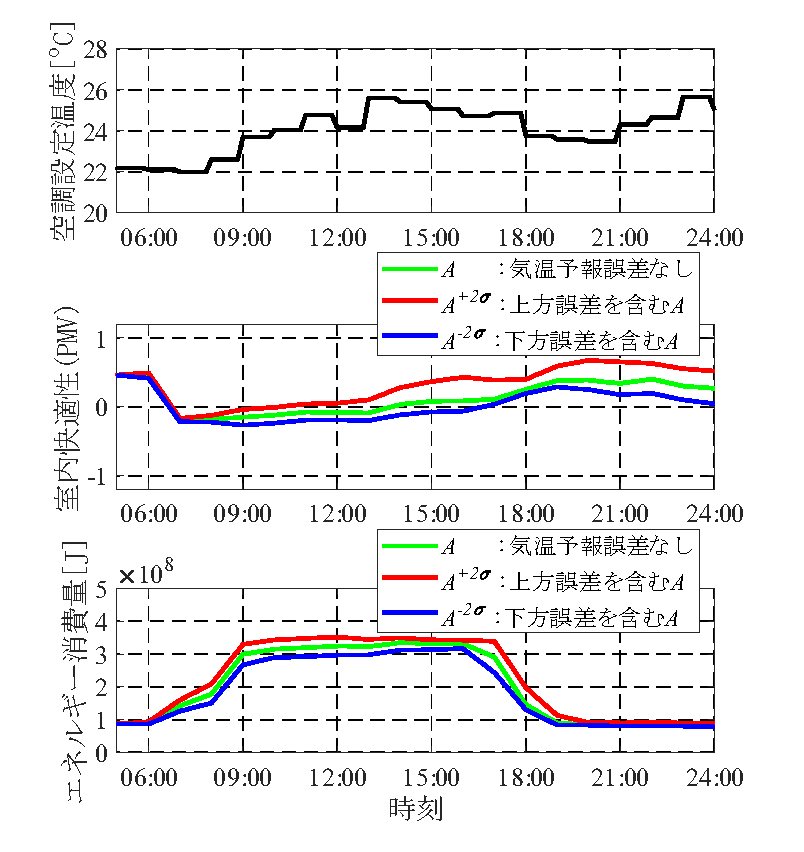
\includegraphics[width=1\textwidth,keepaspectratio=true]{fig/surrogate_result_schedule_robust_4obj.eps}\\\vspace{-5mm}{\small スケジュール X' (ロバスト性を考慮した4目的最適化で得た解)}
      \end{center}
    \end{minipage}
    \vspace{-1mm}
    \caption{サロゲート評価器によって得られた空調設定温度スケジュールの時系列データの例}
    \label{fig::surrogate_result_schedule_robust}
  \end{center}
\end{figure*}

\subsubsection{シミュレーション評価器を用いたロバスト最適化結果との違い}
サロゲート評価器を用いたロバスト最適化が,シミュレーションによるロバスト最適化に対してどれだけ差異を持つかを,(1)目的関数空間上の解分布(2)サロゲート評価器の精度の2つの観点から評価する.\\
(1)目的関数空間上の分布\\
サロゲート評価器を用いたロバスト最適化の結果は,\figref{fig::robust_result_pareto}に示したシミュレーションを用いたロバスト最適化の結果と比較すると,獲得された解分布の傾向は似通っているものの,差異があることがわかった.この違いを詳細に確認するため,各目的関数空間における散布図を散布図行列としてプロットした結果を\figref{fig::surrogate_result_pareto_robust_matrix}に示す.
シミュレーションおよびサロゲート評価器いずれも,ほとんどの目的関数空間で帯状に広がる分布を持っていること,$f_1-f_3$や$f_1-f_4$目的関数空間で目立ったトレードオフ関係が見られないことなど同様の傾向が得られていることがわかる.しかしながら,解集合の分布の範囲が異なる,サロゲート評価器の$f_3-f_4$目的関数空間では2つに別れた分布が見られることなど,差異が見られる.解集合分布は全体としては同様の傾向であることから,これらの際はサロゲート評価器の誤差によるものだと考えられる.そこで,次にサロゲート評価器の予測精度を確認する.\\
(2)サロゲート評価器の精度\\
サロゲート評価器を用いた4目的最適化によって獲得した解集合の分布は,シミュレーションを用いて獲得した解集合と,同様の傾向は示すものの,差異がある.この要因として,サロゲート評価器による解評価精度がロバストな解では悪化していることが考えられる.そこで,まず,サロゲート評価器を用いたロバスト最適化で獲得した解集合を,シミュレーションを用いて評価した解集合と目的関数空間上で比較する.\figref{fig::surrogate_result_pareto_robust_comp}に,サロゲート評価器を用いたロバスト最適化で獲得したスケジュールを黒の丸,同じスケジュール集合をシミュレーションで評価した結果を赤の丸で示す.$f_1-f_2$目的関数空間,$f_3-f_4$目的関数空間どちらとも,サロゲート評価器による評価値とシミュレーションによる評価値の差異が現れており,分布が大きく異なっている.一方で,獲得したスケジュール集合は$f_3-f_4$でもロバストな値を示しており,ロバストな解を探索することはできている.
次に,4目的最適化で獲得したロバストなスケジュールとロバスト性を考慮しない2目的最適化で獲得したスケジュールが,サロゲート評価器による予測誤差がシミュレーションとどれだけ異なるか定量的に評価する.各最適化で獲得したスケジュール集合の時系列データについて,サロゲート評価器とシミュレーションの誤差をMAPEで計算した結果を\tabref{tab::surrogate_predict_robust}に示す.結果から,ロバスト性を考慮した4目的最適化で獲得したスケジュールのサロゲート評価器による誤差は,ロバスト性を考慮していない2目的最適化で獲得したスケジュールよりも,快適性で20倍,エネルギー消費量は5.4倍大きいことがわかった.さらに,外気温予報誤差があると,サロゲート評価器による誤差が1.1\%~6.5\%ほど大きくなる傾向にあることがわかった.これは,サロゲート評価器を学習させる際に,4目的最適化で獲得するようなロバストなスケジュールが学習データにあまり含まれておらず,学習が不足していることが原因であると考えられる.この課題を解消しサロゲート評価器を用いてロバスト最適化をより高精度に実現する方法として,最適化プロセスの途中で,最適化によって獲得した解をシミュレータで評価しサロゲート評価器の学習と更新を逐次的に行う,逐次近似最適化法を適用する方法などが考えられる.
このような手法により,ランダムで生成しただけでは通常得られないロバストなスケジュールに対してもサロゲート評価器の精度の向上と誤差の低減が期待できる.

\begin{figure*}[htbp]
  \begin{center}
    \begin{minipage}{0.8\textwidth}
      \begin{center}
        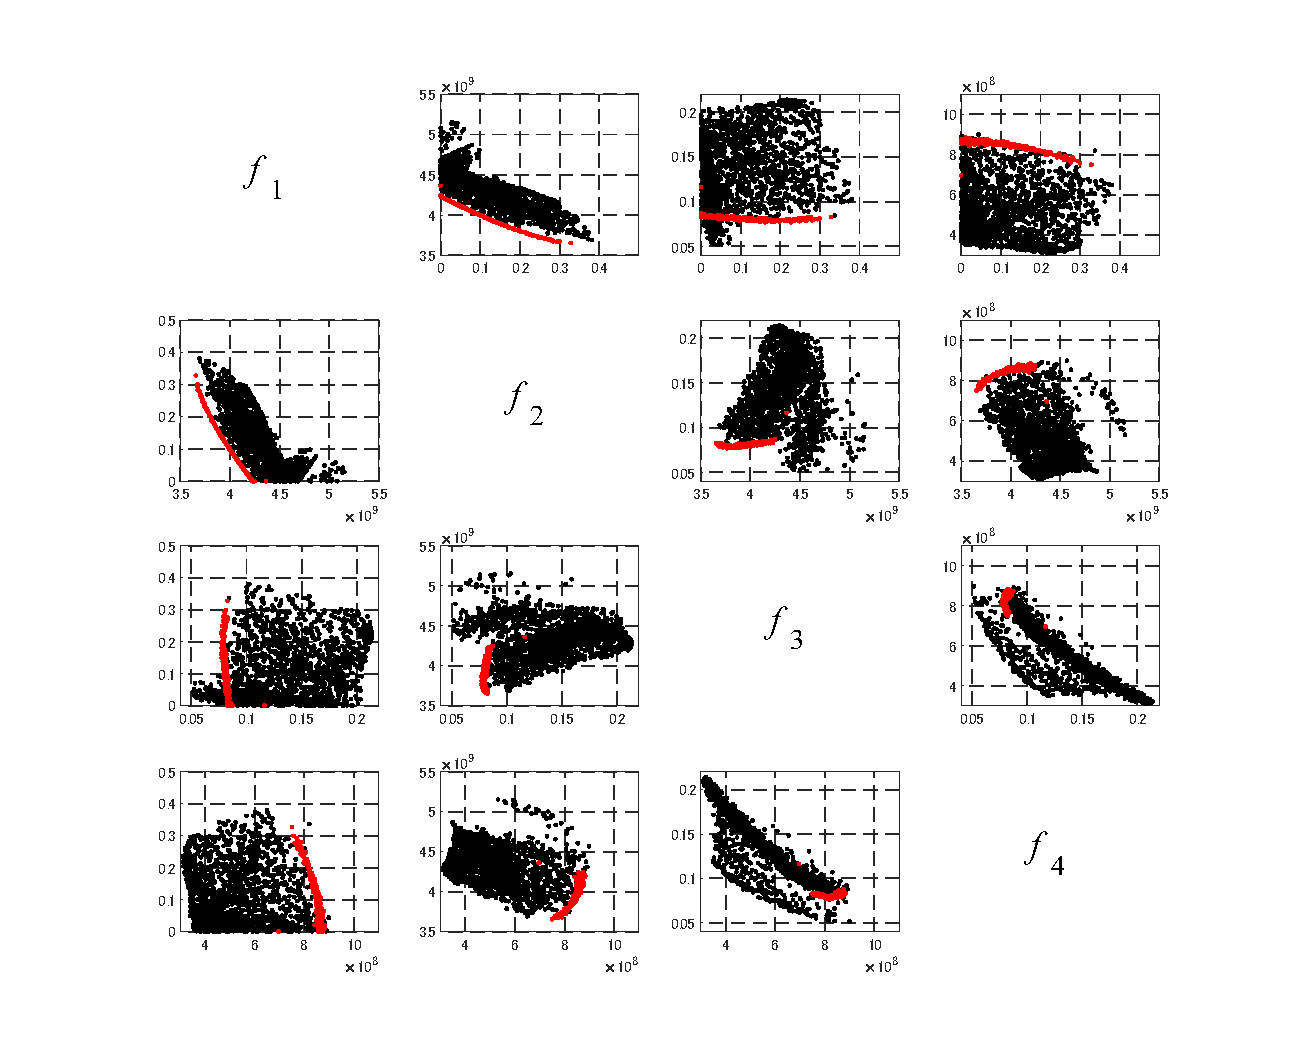
\includegraphics[width=1\textwidth,keepaspectratio=true]{fig/surrogate_result_pareto_robust_matrix_surrogate.eps}\\\vspace{-5mm}{\small (a)サロゲート評価器を用いたロバスト最適化で得た解集合}
      \end{center}
    \end{minipage}
    \\
    \begin{minipage}{0.8\textwidth}
      \begin{center}
        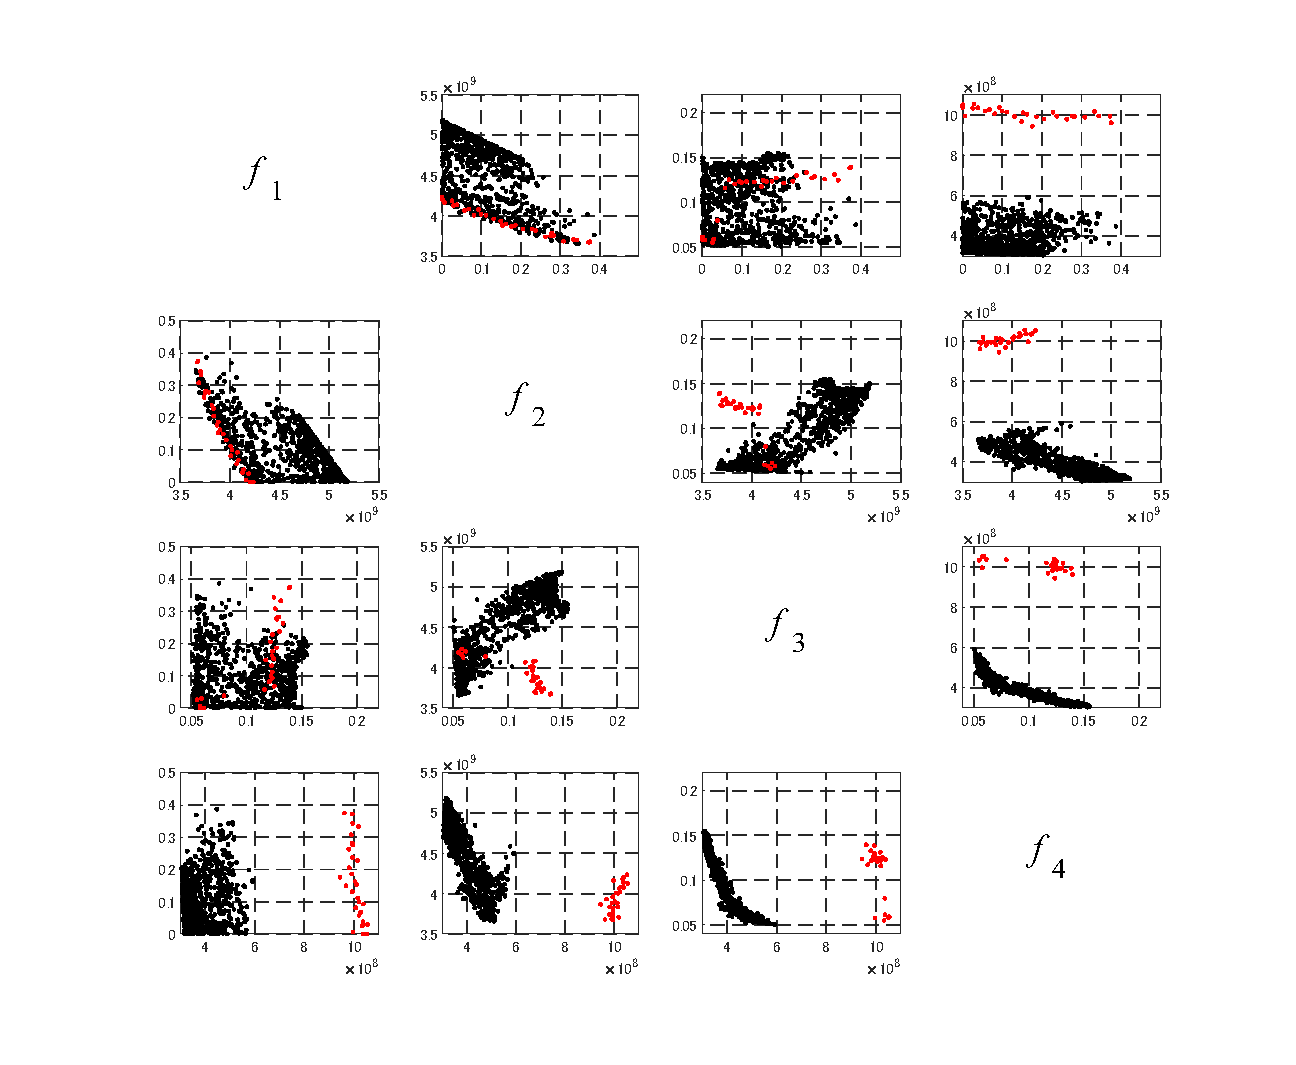
\includegraphics[width=1\textwidth,keepaspectratio=true]{fig/surrogate_result_pareto_robust_matrix_sim.eps}\\\vspace{-5mm}{\small (b)シミュレーションを用いたロバスト最適化で得た解集合}
      \end{center}
    \end{minipage}
    \vspace{-1mm}
    \caption{ロバスト最適化によって得られた空調設定温度スケジュール集合の目的関数空間における散布図行列}
    \label{fig::surrogate_result_pareto_robust_matrix}
  \end{center}
\end{figure*}

\begin{figure*}[htbp]
  \begin{center}
    \begin{minipage}{0.7\textwidth}
      \begin{center}
        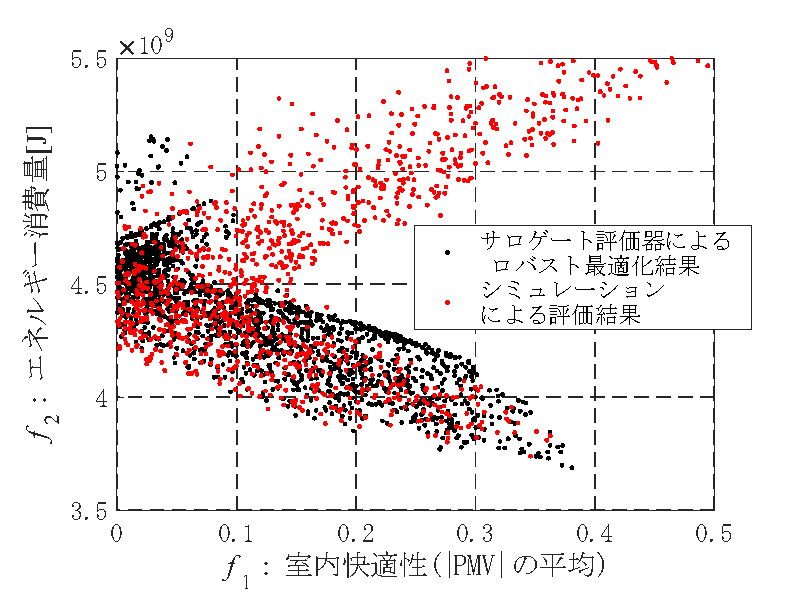
\includegraphics[width=1\textwidth,keepaspectratio=true]{fig/surrogate_result_pareto_robust_comp_f1f2.eps}\\\vspace{-5mm}{\small (a) $f_1$-$f_2$目的関数空間}
      \end{center}
    \end{minipage}
    \\
    \begin{minipage}{0.7\textwidth}
      \begin{center}
        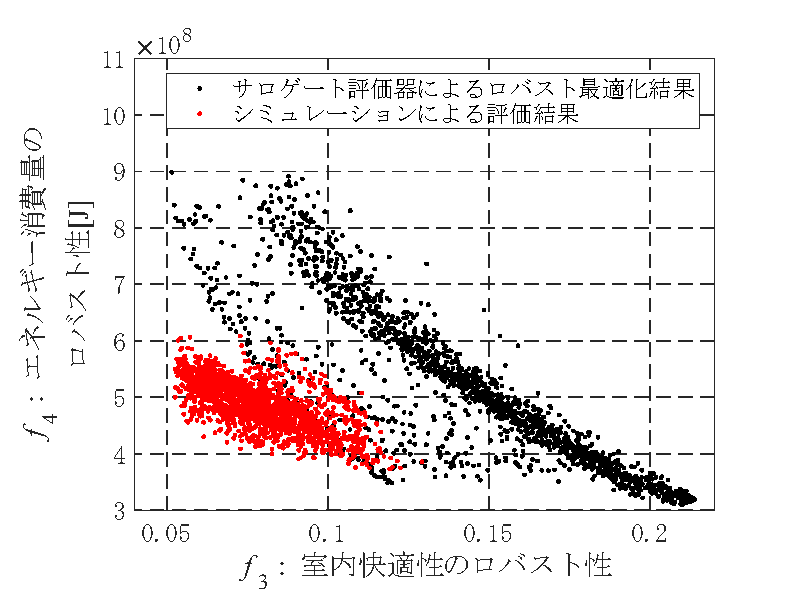
\includegraphics[width=1\textwidth,keepaspectratio=true]{fig/surrogate_result_pareto_robust_comp_f3f4.eps}\\\vspace{-5mm}{\small (B) $f_3$-$f_4$目的関数空間}
      \end{center}
    \end{minipage}
    \vspace{-1mm}
    \caption{サロゲート評価器によって得られたパレート解集合とシミュレーションによる評価結果}
    \label{fig::surrogate_result_pareto_robust_comp}
  \end{center}
\end{figure*}

\begin{table}[t]
  \begin{center}
    \caption{スケジュールおよび気温予報誤差によるサロゲート評価器の予測誤差率(MAPE)}
    \label{tab::surrogate_predict_robust}
    \small
    \begin{tabular}{c|c|c|c}
      \hline
      スケジュール & 気温予報誤差 & 室内快適性のMAPE[\%] & エネルギー消費量のMAPE[\%] \\
      \hline \hline
      2目的最適化  & なし         & 0.48                 & 3.57                       \\
      \cline{2-4}
      で獲得した   & 上方誤差     & 1.27                 & 12.0                       \\
      \cline{2-4}
      スケジュール & 下方誤差     & 0.53                 & 3.26                       \\
      \hline
      4目的最適化  & なし         & 12.3                 & 22.7                       \\
      \cline{2-4}
      で獲得した   & 上方誤差     & 13.0                 & 22.4                       \\
      \cline{2-4}
      スケジュール & 下方誤差     & 13.2                 & 23.5                       \\
      \hline
    \end{tabular}
  \end{center}
\end{table}

\subsubsection{計算時間}
\tabref{tab::surrogate_result_time_robust}に,サロゲート評価器を用いてOMOPSOによるロバスト最適化を行った際の,1つの解の評価時間と,最適化の全体の計算時間を示す.この結果から,1つのスケジュールの評価には,サロゲート評価器はEnergyPlusシミュレーションに対しておおよそ510倍高速となった.加えて,サロゲート評価器による最適化全体の時間は,EnergyPlusシミュレーションの1/93である0.790時間となった.これらの結果から,提案するサロゲート評価器を用いたシステムは空調設定スケジュールのロバスト最適化の高速化が可能であることがわかる.
また,4目的のロバスト最適化におけるサロゲート評価器の高速化の効果は,最適化全体で1/93と,2目的の最適化の1/47よりも大きい.これは,ロバスト最適化では1つの解評価に必要な3回の時系列データの計算を並列化したことが理由であると考えられる.
ロバスト最適化で想定した気温予報誤差は,毎日5:00に発表される気温予報の6:00以降の時刻における誤差であるため,その誤差を考慮した最適化は1時間以内に終えられることが望ましい.サロゲート評価器を用いたロバスト最適化の時間は0.79時間であり,最適化を1時間以内に完了できるため,提案するサロゲート評価器によってロバスト最適化が現実的な時間で実行可能となったと言える.

\begin{table}[t]
  {\footnotesize
    \begin{center}
      \caption{ロバスト最適化の計算時間の比較}
      \label{tab::surrogate_result_time_robust}
      \begin{tabular}{c|cccc}
        \hline
                                 & 従来システム                 & 提案システム                   \\
                                 & (EnergyPlusシミュレーション) & (LSTMに基づくサロゲート評価器) \\
        \hline \hline
        1つの解の平均評価時間    & 110.8 [秒]                   & 0.209 [秒]                     \\
        最適化全体にかかった時間 & 73.6 [時間]                  & 0.790[時間]                    \\
        \hline
      \end{tabular}
    \end{center}
  }
\end{table}

\section{結言}
この章では,空調設定温度スケジュール最適化の高速化のため,時系列予測を行うLSTMに基づくサロゲート評価器を提案した.LSTMベースサロゲート評価器は従来のEnergyPlusシミュレーションの代わりに室内快適性とエネルギー消費量の2つの時系列データを出力する.空調設定温度スケジュールは,この出力された2つの時系列データから算出された目的関数値を用いてOMOPSOによって最適化される.実験結果から,LSTMに基づくサロゲート評価器を用いた提案システムは,室内快適性とエネルギー消費量の間のトレードオフを示す実用的な非劣解を獲得することができた.また,サロゲート評価器によって空調設定スケジュール最適化が47倍高速化されたことを示した.提案するサロゲート評価器は最適化を高速化し高精度な外気温度・外気湿度予報値を使用可能とするため,空調設定温度スケジュールの品質を改善できる.また,本章では,多目的粒子群最適化アルゴリズムOMOPSOの改良手法であるDOMOPSOを提案した.本手法は,従来よりも6.6\%少ない評価回数で同程度の解が探索できる性能を持ち,さらなる最適化の高速化を可能とする.さらに,本章では,5章で述べたロバスト最適化をサロゲート評価器を用いて高速化する手法を提案した.本手法により,ロバスト最適化の時間を従来1/93である0.79時間まで高速化し,現実的な時間で実行できることを示した.
